\documentclass[10pt,a4paper]{article}

\usepackage[margin=0.65in]{geometry}
\usepackage{booktabs}
\usepackage{graphicx}
\usepackage{fancyhdr}
\usepackage[hidelinks]{hyperref}

\graphicspath{{figures/}}
\setlength{\parindent}{0pt}
\setlength{\parskip}{0.35em}
\setlength{\tabcolsep}{5pt}
\renewcommand{\arraystretch}{1.08}
\raggedbottom

\pagestyle{fancy}
\setlength{\headheight}{13pt}
\fancyhf{}
\lhead{Deep Learning Laboratory}
\rhead{Lab Assignment 4}
\cfoot{\thepage}

\newcommand{\resultpanel}[2]{%
    \begin{minipage}{\textwidth}
        \centering
        \includegraphics[width=\textwidth]{#1}
        \vspace{-1mm}
        {\small #2}
    \end{minipage}
    \par\vspace{3mm}
}

\begin{document}

\begin{center}
    {\Large\bfseries Deep Learning Laboratory - Assignment 4}\par
    \vspace{1mm}
    {\small Team 17: Mirthula M (26120121), Karthikeyan M (26120004)}
\end{center}

\section*{Setup}

Network: $36\rightarrow30\rightarrow20\rightarrow5$; ReLU hidden layers; softmax output; five mini-batches; Adam. All studies start from the same weights.

Training stops after five consecutive epochs with $|E_t-E_{t-1}|<10^{-3}$, or at 300 epochs. For L2, the training loss is $\mathrm{CE}+\lambda\sum\|W\|^2/(2N)$.

\section*{Accuracy}

\begin{center}
\small
\begin{tabular}{lrrrr}
\toprule
Method & Epochs & Train (\%) & Val. (\%) & Test (\%)\\
\midrule
No regularization & 300 & 65.55 & 55.00 & 52.20\\
L2, $\lambda=0.1$ & 300 & 64.20 & 52.80 & 52.60\\
L2, $\lambda=1.0$ & 300 & 61.90 & 53.00 & \textbf{53.60}\\
L2, $\lambda=10.0$ & 151 & 49.70 & 47.00 & 49.00\\
Dropout, 10\% & 300 & 68.60 & 49.00 & 50.40\\
Dropout, 20\% & 300 & 67.90 & 52.80 & 48.20\\
Dropconnect, 5\% & 300 & 60.45 & \textbf{55.40} & 53.20\\
Dropconnect, 10\% & 300 & 57.15 & 54.40 & 51.40\\
Post-activation batch norm & 300 & 81.15 & 44.20 & 45.80\\
\bottomrule
\end{tabular}
\end{center}

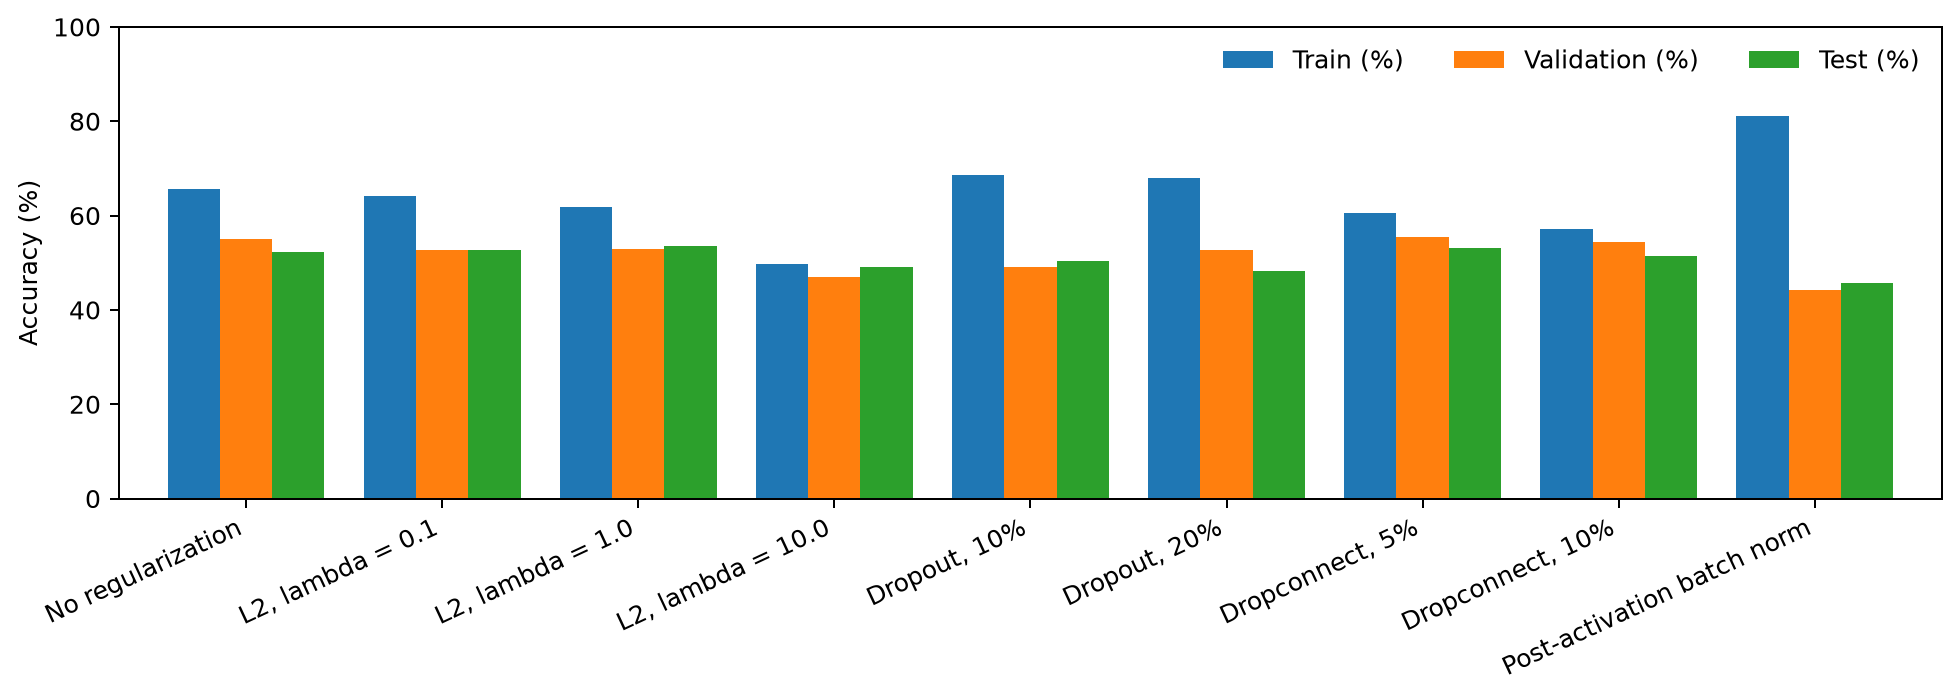
\includegraphics[width=\textwidth]{accuracy_summary.png}

\textbf{Result.} Dropconnect at 5\% gives the best validation accuracy. L2 with $\lambda=1$ gives the best test accuracy. Strong L2 and batch normalization reduce generalization here.

\clearpage
\section*{Error curves and confusion matrices}

\resultpanel{no_regularization.png}{No regularization provides the reference result.}
\resultpanel{l2_0_1.png}{Light L2 gives similar test accuracy.}
\resultpanel{l2_1_0.png}{L2 with $\lambda=1$ gives the highest test accuracy.}

\clearpage
\resultpanel{l2_10_0.png}{Strong L2 causes underfitting.}
\resultpanel{dropout_10.png}{Dropout at 10\% lowers validation accuracy.}
\resultpanel{dropout_20.png}{Dropout at 20\% lowers test accuracy.}

\clearpage
\resultpanel{dropconnect_05.png}{Dropconnect at 5\% gives the highest validation accuracy.}
\resultpanel{dropconnect_10.png}{Dropconnect at 10\% remains close to the baseline.}
\resultpanel{batch_norm.png}{Batch normalization overfits this training split.}

\end{document}
